\section{Wellenleiter}
\subsection{Koaxial Leiter}
\subsubsection{Wellenwiderstand}

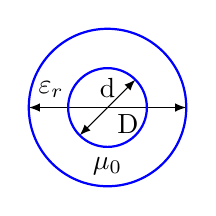
\begin{tikzpicture}
    \draw[latex-latex](-1,0)node[above right]{$\varepsilon_r$}--(1,0);
    \node[below right, yshift=1pt]{D};
    \draw[latex-latex, rotate=45](-0.5,0)--(.5,0);
    \node at (0,0)[above]{d};
    \draw[-, thick, blue](0,0) circle (1);
    \node at(0,-.75)[]{$\mu_0$};
    \draw[-, thick, blue](0,0) circle (0.5) ;
\end{tikzpicture}

\begin{align*}
	\Aboxed{Z_L & = \frac{Z_{F0}}{2\pi}\sqrt{\frac{\mu_r}{\varepsilon_r}}\ln\left( \frac{r_a}{r_i} \right)}  \overbrace{=}^{ \mu_r=1}\frac{60\Omega}{\sqrt{\varepsilon_r}}\cdot \ln{\frac{r_a}{r_i}}
\end{align*}

\subsubsection{Dämpfung}
Hin- und Rückleiter!

\underline{\textbf{Ohmsche Verluste}} $R\ll\omega L$
\[
	\alpha_L = \frac{\sqrt{\dfrac{f\cdot\mu}{\pi\cdot\kappa}}}{120\Omega}\cdot\frac{\sqrt{\varepsilon_r}}{D}\cdot\dfrac{1+\dfrac{D}{d}}{\ln \dfrac{D}{d}}
\]

Dämpfungsminimum für $ \frac{1+\tfrac{D}{d}}{\ln \tfrac{D}{d}} = 1 $

Bei vorgegebenen Außendurchmesser: $ \frac{D}{d} =3,59 $

\vspace{1em}
\underline{\textbf{Dielektrische Verluste}} $G\ll\omega C$, $\tan\delta=
	(^G/_{\omega C})$
\[
	\alpha_d = \frac{\sqrt{\varepsilon_r}\pi f}{c_0}\cdot\tan\delta \sim f
\]

\subsection{Mikrostreifenleiter}
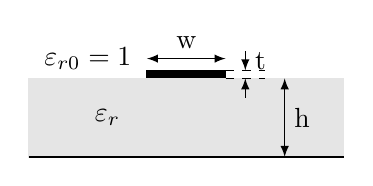
\begin{tikzpicture}
    %Leiterbahn
    \filldraw[black]    (1,1)   rectangle (2,1.1);
    %Dielektrika
    \filldraw[black!10] (-.5,0) rectangle (3.5,1);
    \draw[-,thick](-.5,0)--(3.5,0);
    %Bemassungen
    \draw[latex-latex](2.75,0)--(2.75,1) node[midway, right]{h};
    \draw[latex-latex](1,1.25)--(2,1.25) node[midway, above]{w};
    \draw[dashed](2,1)      --(2.5,1);
    \draw[dashed](2,1.1)    --(2.5,1.1);
    \draw[latex-](2.25,1)   --(2.25,.75);
    \draw[latex-](2.25,1.1) --(2.25,1.35) node[midway, right]{t};
    %Dielektrizitätskonstanten
    \node at (.5,.5)[]{$\varepsilon_r$};
    \node at (.25,1.25)[]{$\varepsilon_{r0}=1$};
\end{tikzpicture}


\subsubsection{Effektive Permittivitätszahl}
Unterschiedliche Phasengeschwindigkeit $\rightarrow$ Dispersion
Je größer $\dfrac{\mathrm{w}}{\mathrm{h}}$ desto mehr nähert sich
$\varepsilon_{r,\texttt{eff}}$ an $\varepsilon_r$ und
\[
	\lambda = \frac{\lambda_0}{\sqrt{\varepsilon_{r,\texttt{eff}}\cdot\mu_{r,\texttt{eff}}}}
\]

\subsubsection[Schmale Streifen]{Schmale Streifen (ca 20-200$\Omega$) $\frac{\mathrm{w}}{\mathrm{h}}\leq 1$}
\[
	\varepsilon_{r,\texttt{eff}}  = \frac{\varepsilon_r+1}{2} + \frac{\varepsilon_r-1}{2}
  \left[\frac{1}{\sqrt{1+12\cdot\frac{\mathrm{h}}{\mathrm{w}}}} +
  0,04\cdot\left(1-\frac{\mathrm{w}}{\mathrm{h}}\right)^2\right]
\]

\[
	Z_L = \frac{60\Omega}{\sqrt{\varepsilon_{r,\texttt{eff}}}}\cdot\ln\left(\frac{8\mathrm{h}}{\mathrm{w}}+\frac{\mathrm{w}}{4\mathrm{h}}\right)
\]

\subsubsection[Breite Streifen]{Breite Streifen (ca 20-200$\Omega$) $\frac{\mathrm{w}}{\mathrm{h}} > 1$}
\[
	\varepsilon_{r,\texttt{eff}}  = \frac{\varepsilon_r+1}{2} + \frac{\varepsilon_r-1}{2}
  \left[\frac{1}{\sqrt{1+12\cdot\frac{\mathrm{h}}{\mathrm{w}}}}\right]
\]

\[
	Z_L = \frac{120\pi\Omega}{\sqrt{\varepsilon_{r,\texttt{eff}}}}\cdot\frac{1}{\dfrac{\mathrm{w}}{\mathrm{h}}+2,42-0,44\cdot\dfrac{\mathrm{h}}{\mathrm{w}}+\left(1-\dfrac{\mathrm{h}}{\mathrm{w}}\right)^6}
\]

\subsection{Hohlleiter}
\[
	f_c = \frac{c_0}{2a}
\]

\subsection{VSWR (Voltage Standing Wave Ratio) und Return Loss}\label{sec:VSWR}

Überlagerung von einlaufender und reflektierender Welle. Wenn Transmission
vorhanden $\rightarrow$ Teil der Welle wird an der Grenzfläche transmittiert.
Abhängigkeit vom Reflexionsfaktor.

\textbf{Reflexionsfaktor}
\[
	\underline{r}_2 = \underline{r}(z=0) = \frac{Z_2 - \underline{Z}_L}{Z_2 + \underline{Z}_L}
\]

\underline{VSWR}
\begin{align*}
	s   & = \mathrm{VSWR} = \frac{1+|r|}{1-|r|}\geq 1 \\
	|r| & = \frac{s-1}{s+1}
\end{align*}

\underline{Return Loss}
\[
	\alpha_r = -20\log(r)dB
\]

\underline{Missmatch Loss}
\[
	\mathrm{ML} = -10\log(1-r^2)dB
\]

\subsection{Lichtwellenleiter oder Glasfaser}
\begin{description}
	\setlength\itemsep{1pt}
	\item APF := All Plastic Fiber
	\item POF := Polymerfaser
	\item LWL := Lichtwellenleiter
	\item $B\cdot l$ := Bandbreitenlängenprodukt
\end{description}

\begin{description}
	\item \underline{Dispersion:}\\
	      {\small Die von der Frequenz des Lichts abhängende
	      Ausbreitungsgeschwindigkeit des Lichts in Medien. Dies hat zur Folge,
	      dass Licht an Übergangsflächen unterschiedlich stark gebrochen wird.
	      Somit verflacht sich beispielsweise ein (Dirac-)Impuls zu einer Gauß'schen
	      Glocke.
	      }

	\item \underline{Stufenprofil:}\\
	      {\small Multimode: leichtes Einkoppeln, geringes $B\cdot l$ wegen
	      Modendispersion

	      Single/Monomode: schwieriges Einkoppeln, großes $B\cdot l$, keine
	      Modendispersion
	      }

	\item \underline{Gradientenprofil:}\\
	      {\small Multimode: Kompromiss beim Einkoppeln und Reichweite mit $B\cdot l$}

	\item \underline{Bandbreitenlängenprodukt:}\\
	      {\small $B' =  B\cdot l[\frac{MHz}{km}]$ = konstant

	      $B \sim \frac{1}{l}$ und $l\sim \frac{1}{B}$

	      Bandbreite ist gegen Übertragungslänge austauschbar, solange
	      Dämpfung keine Rolle spielt.
	      }
\end{description}

